\documentclass[tikz, border=2pt]{standalone}
\usepackage{tikz}
\begin{document}
    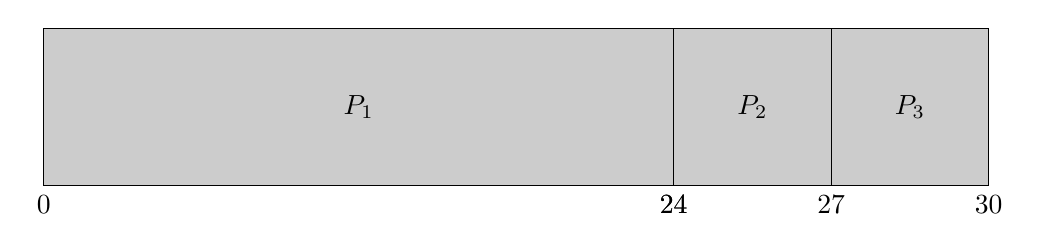
\begin{tikzpicture}
        \draw [fill=black!20] (0,0) rectangle (8,2) 
            node [midway] {$P_1$} 
            node [pos=0, below] {0}
            node at (8,0) [below] {24};
        \draw [fill=black!20] (8,0) rectangle (10,2) node [midway] {$P_2$}
            node [pos=0, below] {24}
            node at (10,0) [below] {27};
        \draw [fill=black!20] (10,0) rectangle (12,2) node [midway] {$P_3$}
            node at (12,0) [below] {30};
    \end{tikzpicture}
\end{document}